% Created 2014-12-17 Wed 16:24
\documentclass[11pt]{template/openetcs_report}
\usepackage{fixltx2e}
\usepackage{graphicx}
\usepackage{longtable}
\usepackage{float}
\usepackage{wrapfig}
\usepackage{rotating}
\usepackage[normalem]{ulem}
\usepackage{amsmath}
\usepackage{textcomp}
\usepackage{marvosym}
\usepackage{wasysym}
\usepackage{amssymb}
\usepackage{hyperref}
\tolerance=1000
\usepackage{todonotes}
\usepackage{pdfpages}
\hypersetup{
  pdfkeywords={},
  pdfsubject={},
  linkbordercolor 	= {1 1 1},
  pdfcreator={Emacs 24.3.1 (Org mode 8.2.4)}}
%===========================
% Graphicpath
%===========================
\graphicspath{{./template/}{.}{./images/}}
%===========================
% Todo note margin
%===========================
\setlength{\marginparwidth}{7em}
%\let\oldmarginpar\marginpar
%\renewcommand\marginpar[1]{\-\oldmarginpar[\raggedleft\footnotesize #1]%
%{\raggedright\footnotesize #1}}
%===========================


\begin{document}
\frontmatter
\project{openETCS}


%assign a report number here
\reportnum{OETCS/WP7/07.3.5}

%define your workpackage here
\wp{Work-Package 7: ``Toolchain''}

%set a title here
\title{OpenETCS Roadmap}

%set a subtitle here
%\subtitle{}

%set the date of the report here


\date{\today}
\title{Traceability Architecture in OpenETCS}
\subtitle{WP7 Proposition}
%define a list of authors and their affiliation here

\creatorname{Cécile Braunstein}
\creatoraffil{University Bremen}
\techassessorname{}
\techassessoraffil{}

\qualityassessorname{}
\qualityassessoraffil{}

\approvalname{}
\approvalaffil{}
\author{Cecile Braunstein}
\affiliation{University Bremen}

\author{Moritz Dorka}
\affiliation{DB}

\author{David Mentré}
\affiliation{Mitsubishi Electric R\&D Centre Europe}

\author{Raphaël Faudou}
\affiliation{Samares Engineering on behalf of ENSEEIHT}


% define the coverart
\coverart[width=350pt]{openETCS_EUPL}

%define the type of report
\reporttype{OpenETCS : Position Paper on traceability}


\begin{abstract}
%define an abstract here
This document presents a propostion to the tool chain traceability
architecture.
\end{abstract}


\maketitle
\tableofcontents

\newpage
%=============================

% The actual document starts below this line
%=============================
%Start here
%=============================
% Document Managment
%=============================
\chapter{Document Information}

\begin{tabular}{|p{4.4cm}|p{8.7cm}|}
\hline
\multicolumn{2}{|c|}{Document information} \\
\hline
Work Package &  WP7  \\
Deliverable ID or doc. ref. & O7.3.5\\
\hline
Document title &Traceability Architecture in OpenETCS \\
Document version & 00.02 \\
Document authors (org.)  & Cécile Braunstein (Uni.Bremen) \\
\hline
\end{tabular}

\begin{tabular}{|p{4.4cm}|p{8.7cm}|}
\hline
\multicolumn{2}{|c|}{Review information} \\
\hline
Last version reviewed &  \\
\hline
Main reviewers &  \\
\hline
\end{tabular}

\begin{tabular}{|p{2.2cm}|p{4cm}|p{4cm}|p{2cm}|}
\hline
\multicolumn{4}{|c|}{Approbation} \\
\hline
  &  Name & Role & Date   \\
\hline  
Written by    &  Cécile Braunstein & WP7-T7.3 Sub-Task  & 06.02.2014 \\
&  & Leader&\\
\hline
Approved by &  &   &  \\
\hline
\end{tabular}

\begin{tabular}{|p{2.2cm}|p{2cm}|p{3cm}|p{5cm}|}
\hline
\multicolumn{4}{|c|}{Document evolution} \\
\hline
Version &  Date & Author(s) & Justification  \\
\hline  
00.00 & 17.12.2014 & C. Braunstein  &  Document creation  \\
\hline  
00.00 & 23.10.2015 & R. Faudou  &  Precisions concerning OpenETCS requirements and models and update of tool chain traceability requirements  \\


\hline  
\end{tabular}
\newpage
%==========================================
\mainmatter
%----------------------
\chapter{OpenETCS traceability scope}

Requirements traceability concerns relations between requirements existing at different engineering levels and relations between requirements and other engineering artefacts (models, documents, test cases, code...). All those requirement traceability links can have different semantics including derivation, refinement,  satisfaction, implementation and verification. 

Before defining traceability process and the different link types, it is important to clearly define the scope of the requirements and of the models that we want to trace in openETCS project.
Next paragraphs recall the different engineering levels defined by ISO 15288:2015 (standard concerning systems life cycle) and position OpenETCS requirements, models and documents with regards to those engineering levels.

\section{OpenETCS requirements with regards to standard engineering levels}
\label{sec-1}
ISO 15288:2015 defines 3 main generic levels: 
\begin{itemize}
\item problem definition,
\item system/Sub system definition (recursive decomposition) 
\item physical building blocks of software, hardware (mechanical, electrical, electronics, plastic...) or procedures that can be realized independently and integrated to provide whole system
\end{itemize}

\begin{figure}[htb]
\centering
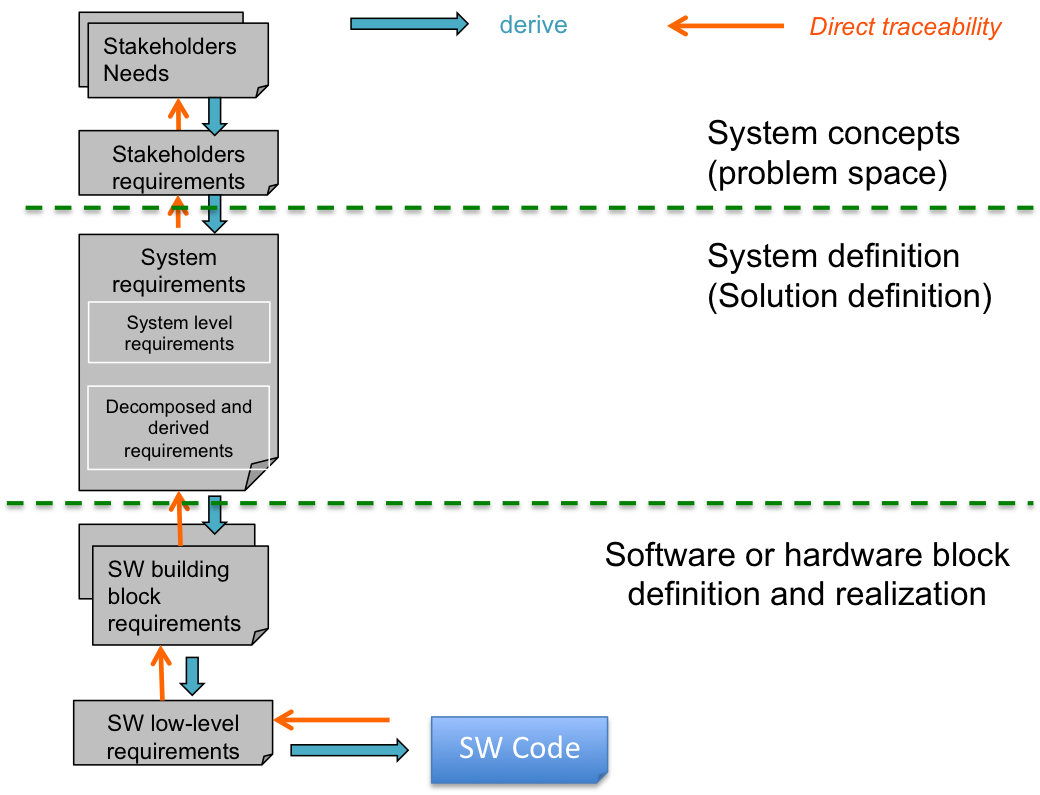
\includegraphics[width=.9\linewidth]{./images/standardRequirementEngineering.png}
\caption{\label{fig:standardReqEngineering}IS0 15288:2015 standard Systems Engineering requirement levels}
\end{figure}

Concerning OpenETCS project, there are 5 main sources for requirements:
\begin{itemize}
\item User stories, concerning problem definition
\item CENELEC regulation requirements that are part of stakeholder requirements
\item SRS Subset 026 that can be considered as system level requirements
\item openETCS new requirements created during system definition by decomposition or derivation of SRS Subset 026 requirements
\item openETCS API, that provides software requirements to integrate a vendor specific platform
\end{itemize}


\begin{figure} [htb]
\centering
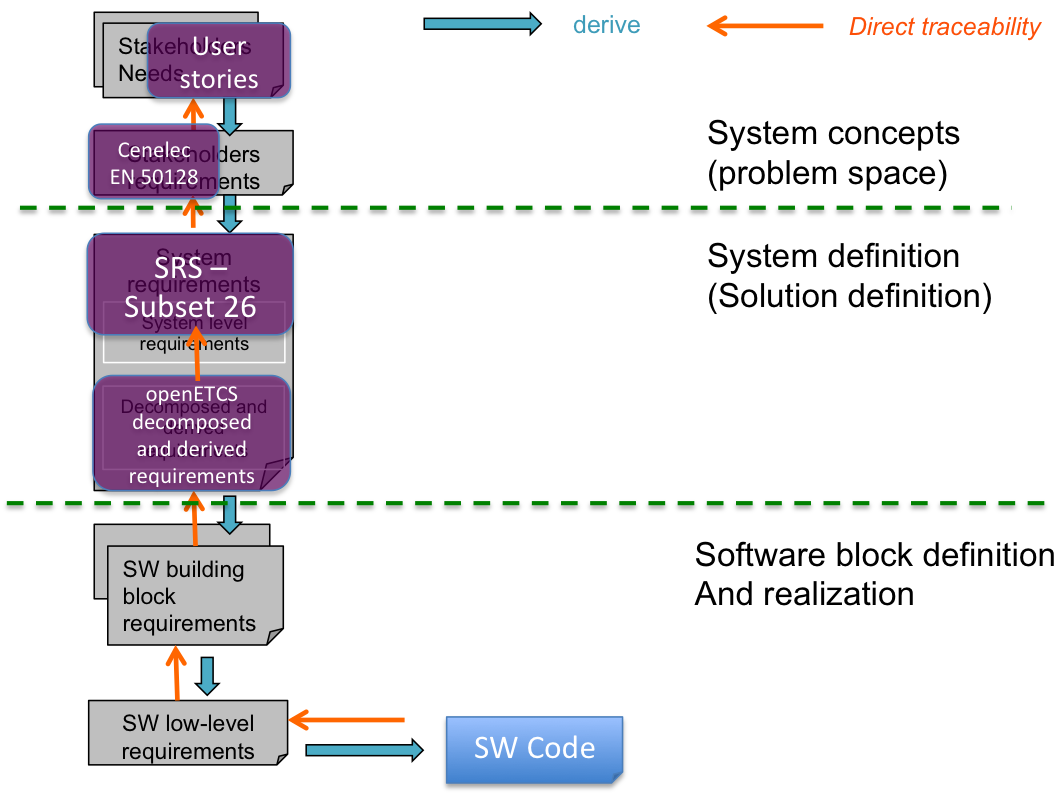
\includegraphics[width=.9\linewidth]
{./images/OpenETCSRequirementsWrtStandard.png}
\caption{\label{fig:OpenETCSRequirementsWrtStandard}OpenETCS requirements with regards to standard engineering levels}
\end{figure} 


\section{OpenETCS models with regards to requirement engineering levels}
\label{sec-2}

Models can be used for different purposes including illustration of concepts, operational scenarios, formalization of requirements, product breakdown structure... and can have different scopes. Figure \ref{fig:requirementEngineeringWithModels}
shows a possible classification of models aligned on the standard requirement engineering levels introduced in previous paragraph.

\begin{figure}[htb]
\centering
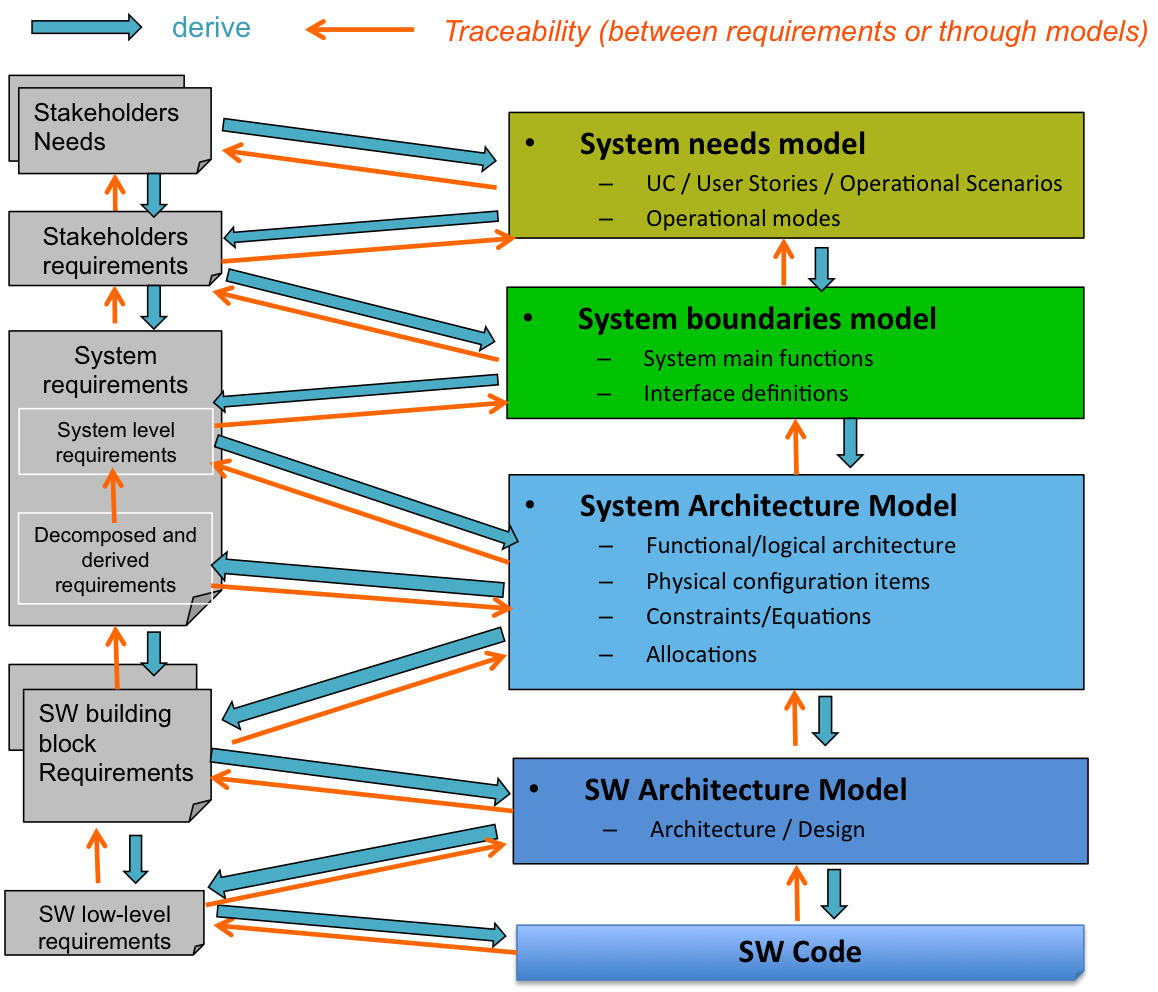
\includegraphics[width=.9\linewidth]
{./images/requirementEngineeringWithModels.png}
\caption{\label{fig:requirementEngineeringWithModels}Possible classification of models with respect to standard requirement engineering levels}
\end{figure}

Figure \ref{fig:openETCSRequirementsAndModels} illustrates the different models produced in the openETCS project and positionned on standard engineering levels:
\begin{itemize}
\item User stories model that refines user stories 
\item OpenETCS EVC model, that describes system breakdown structure with system elements (including ETCS OnBoard Unit) and their interfaces
\item Data dictionary model, that stores all messages, data and functions used in architecture interface definitions
\item OpenETCS Onboard Unit functions model, a formal executable model that focuses on ETCS Kernel functions addressed in Subset026 SRS
\end{itemize}

 
\begin{figure}[htb]
\centering
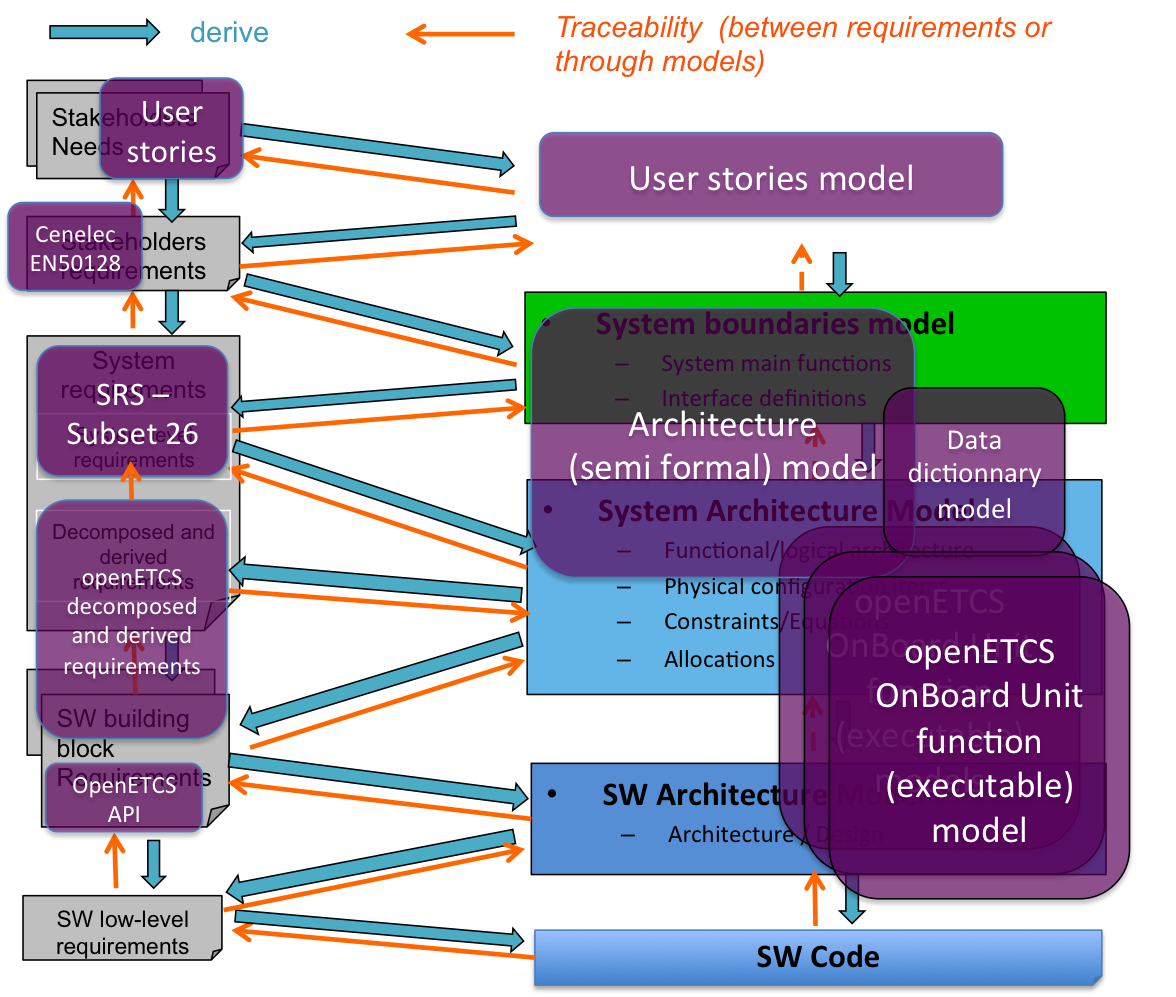
\includegraphics[width=.9\linewidth]
{./images/openETCSRequirementsAndModels.png}
\caption{\label{fig:openETCSRequirementsAndModels}OpenETCS requirements and models with respect to standard requirement engineering levels}
\end{figure}

\chapter{OpenETCS traceability priorities and expectations}
\section{Traceability priorities}
\label{sec-3-1} 
Most important traceability chain concerns links between ETCS OBU functions model and Subset026 SRS requirements and all other requirements created during system analysis, either by decomposition, refinement or derivation. 
ETCS OBU functional model is detailed down to software level, and as it is a formal model, it becomes possible to generate code from that model. So, if it is possible to demonstrate that this model satisfies some Subset026 SRS requirements, then it will be possible to establish that software code generated from that model also satisfies those requirements.

Other "nice to have" traceability chains concern system model and data dictionary model. Those models need to be traced to Subset026 SRS requirements in order to ensure that they are representative of OpenETCS system and are complete (all requirements are covered, no missing requirement). 

Figure \ref{fig:openETCSTraceabilityMainPriority} highlights traceability chains with highest priority (arrows with largest size).

\begin{figure}[htb]
\centering
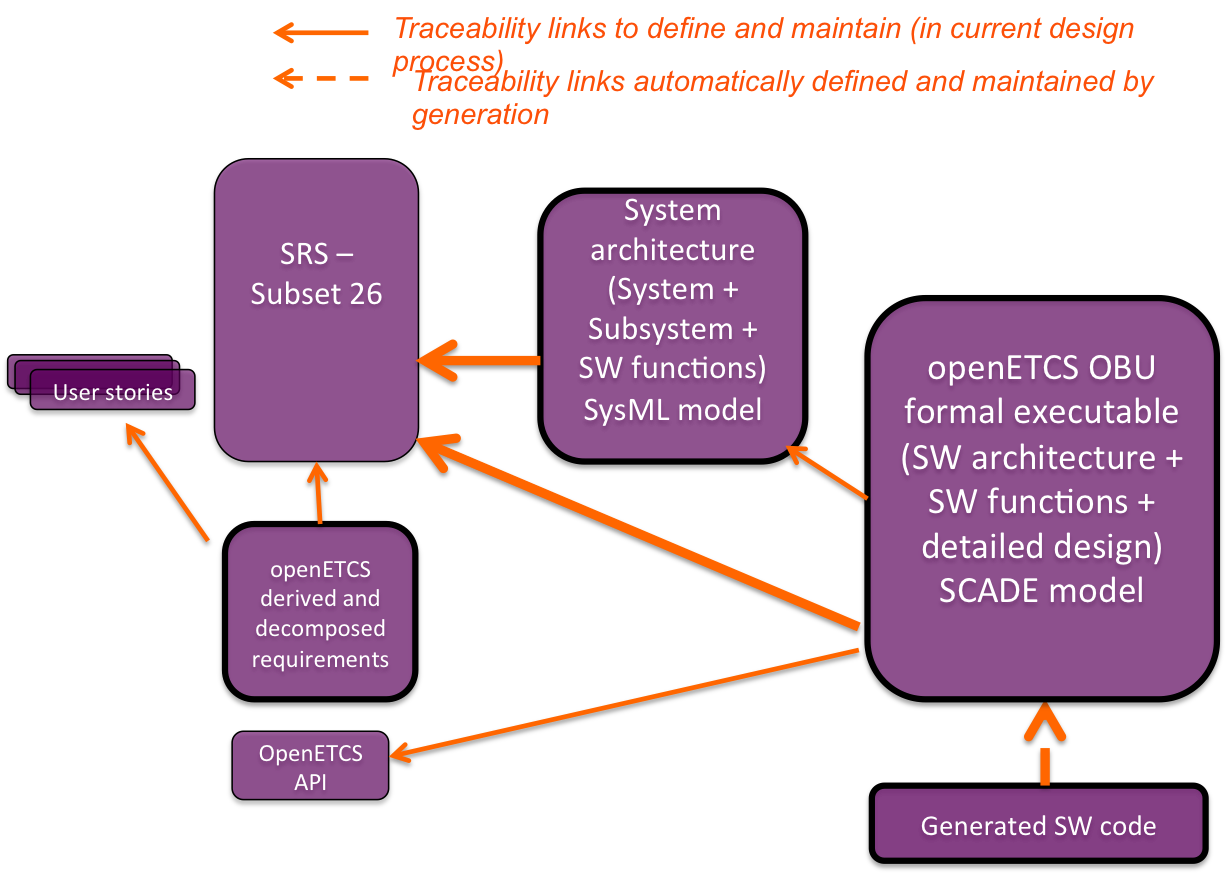
\includegraphics[width=.9\linewidth]
{./images/openETCSTraceabilityMainPriority.png}
\caption{\label{fig:openETCSTraceabilityMainPriority}OpenETCS traceability chains with highest priority}
\end{figure}

\section{Traceability expectations}

\subsection{Traceability Process}
\label{sec-2-2-1}
From the Subset026 SRS specification we want to be able to trace all artifacts
that implement it.
\begin{figure}[htb]
\centering
\includegraphics[width=.9\linewidth]{./images/trace_archi.pdf}
\caption{\label{fig:trace_process}Traceability architecture between artifacts}
\end{figure}

Figure  \ref{fig:trace_process} highlights the different artifacts or activities and their
links. Traceability activities should allow to trace a requirement within all
the artifacts and/or activities that are using it.

The goal of traceability is that, from any artifacts produced, we are able to
track which requirement it realizes, implements  or refers to. These links can
take different form and be done by different tools. 

\subsection{OpenETCS traceability main scenario}
\label{sec-2-2-2}

Here is a global scenario that illustrates the way an OpenETCS system designer will manage existing reference requirements and will create new ones by decomposition or derivation to a lower engineering level,how he/she will provide a functional solution (functional model) to satisfy the different OpenETCS requirements and verification means (tests or else) to verify them.
\begin{figure}[htb]
\centering
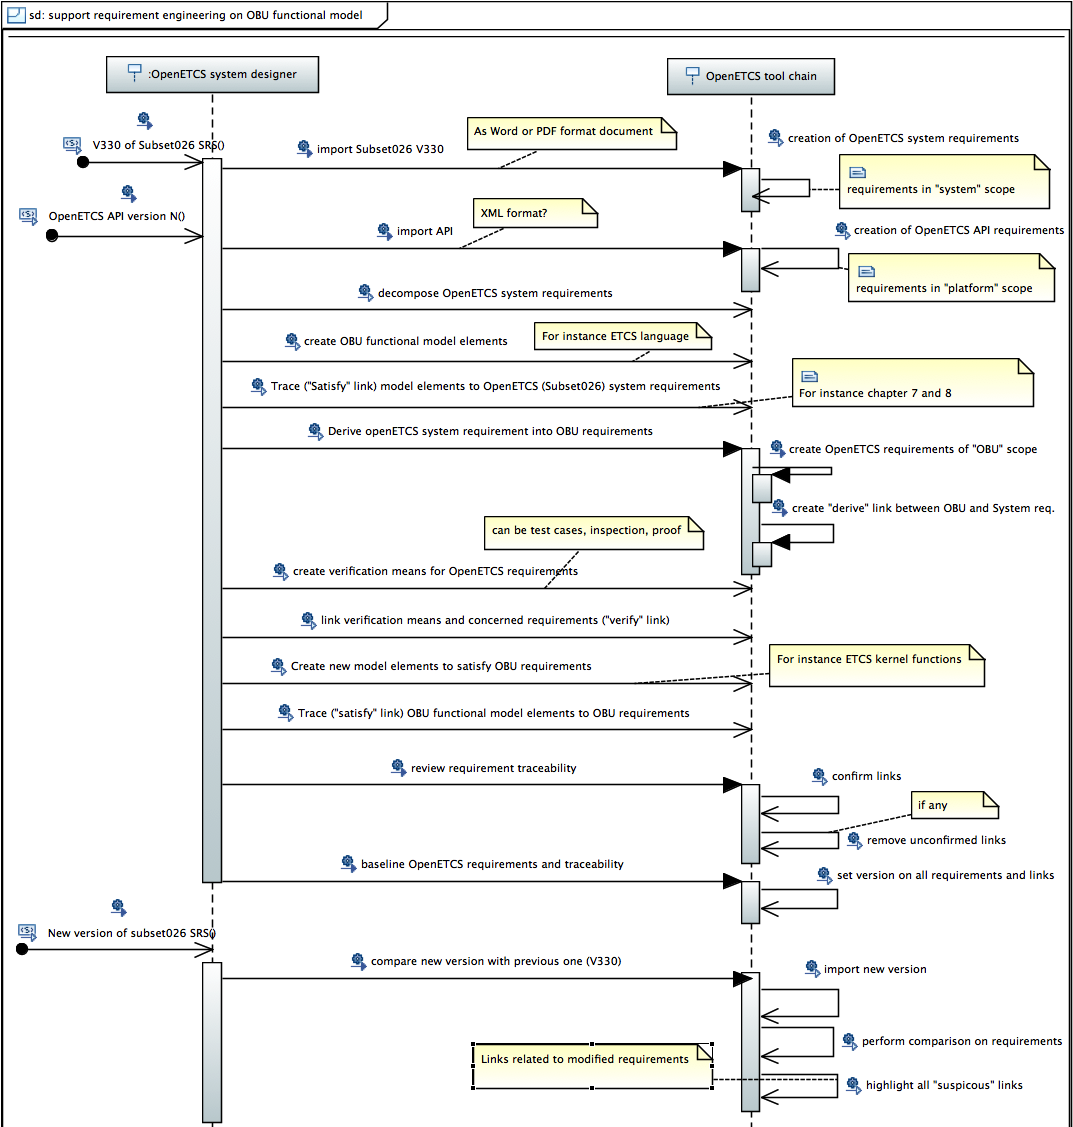
\includegraphics[width=1.0\linewidth]{./images/ToolChainTraceabilityMainScenario.png}
\caption{\label{fig:toolChainTraceabilityMainScenario}Main traceability scenario concerning tool chain }
\end{figure}




\chapter{OpenETCS tool chain requirements about traceability}
\label{sec-3} 
Requirement traceability cannot be fully supported by tool chain if there is no ability to manage requirements (create, edit, visualize, classify...) as expressed in previous chapter through traceability process and main scenario.
Next paragraphs define tool chain capabilities required to support requirement management and requirement traceability in the context of OpenETCS expectations presented previously.

\section{Tool chain capabilities to support requirement management}

Requirement management is an activity that consists in supporting different tasks concerning requirements during the project, whatever the engineering level. In OpenETCS project we need at least the following commands available in the tool chain (and potentially restricted according to access rights if defined):
\begin{itemize}

\item Visualization of one or several requirements, their links if any and their attributes. 
\begin{itemize} \item \textbf{OpenETCS example}: visualize one Subset026 SRS or API requirement, its statement and its hierarchy (father requirement if any and children requirements if any).\end{itemize}

\item Query (filter, ordering) on a set of requirements with filter based on requirement attribute values or on links between requirements
\begin{itemize} \item \textbf{OpenETCS example}: list only subset026 SRS chapter 7 requirements that are not yet traced (no traceability link).\end{itemize}

\item Creation and storage of requirement and of different attributes based on a given requirement template/type, in a given requirement hierarchy and with unique identifier allocation based on a flexible (customizable) strategy
\begin{itemize} \item \textbf{OpenETCS example}: creation of a new openETCS requirement decomposed from a susbet026 SRS requirement. Newly created requirement shall have unique identifier automatically allocated to be consistent with its hierarchy (father requirement id) and with an attribute "maturity" set to "to be confirmed" and creation date set to the current date.\end{itemize}

\item classification of one or several requirements into modules/groups that can be defined by end users.
\begin{itemize} \item \textbf{OpenETCS example}: allocation of a newly created requirement to the Onboard Unit scope.\end{itemize}

\item Edition of one or several requirements and their attributes
\begin{itemize} \item \textbf{OpenETCS example}: confirmation of a newly created requirement with attribute "maturity" set to "confirmed".\end{itemize}

\item Addition of a version on one requirement or on a set of requirements
\begin{itemize} \item \textbf{OpenETCS example}: selection of a set of reviewed openETCS requirements and addition of a version for all those requirements.\end{itemize}

\item Ability to compare two versions of a set of requirements and list all requirements that have been added or modified.
\begin{itemize} \item \textbf{OpenETCS example}: comparison of two versions of Subset026 SRS requirements and visualization of all requirement links to check.\end{itemize}

\item Import of requirements coming from external sources (ReqIF, Word, Excel...)
\begin{itemize} \item \textbf{openETCS example}: import of Subset026 Word document or ReqIF format. Import of openETCS API definition.\end{itemize}

\item Export of a set of requirements to another format: at least ReqIF standard interchange format but also office format (.csv, excel or word...) \begin{itemize} \item \textbf{OpenETCS example}: export of all openETCS created requirements and links into .csv file \end{itemize}

\end{itemize}

In addition, requirement management tooling shall enable share and access of requirements within a team, through a shared repository (shared directory on a network drive or CVS repository like SVN, Git, ClearCase or any other one): either directly (all team members access same shared repository) or with local work and synchronizations between team members through a shared repository.

\section{Tool chain capabilities to support requirement traceability}
\label{sec-3-2}  
Requirement traceability activity consists in ensuring that all product engineering artefacts (including verification means) can be traced to an originating stakeholder requirement either directly (direct link) or through other system requirements derived from stakeholder requirements. It means creating links but also manage their status (created, confirmed...) and potentially their deletion.

In order to support this activity in openETCS project we need at least the following commands available in the tool chain:

\begin{itemize}

\item Creation of a link between a requirement and an engineering artefact, based on a given link template/type (refine, derive, implement, verify...). 
\begin{itemize} \item \textbf{OpenETCS example}: create a "Satisfy" link between one Subset026 SRS requirement and one OnBoard Unit function, with  "status" link attribute set to "defined" and "rationale" attribute set with appropriate justification.\end{itemize}

\item edition of link status. 
\begin{itemize} \item \textbf{OpenETCS example}: after review, confirm some traceability links  by setting "status" attribute to "validated" value.
	\item \textbf{other OpenETCS example}: after change in some Subset026 SRS requirements, for all traceability links of modified requirements, set status to "to check" value.\end{itemize}

\item deletion of requirement traceability link. 
\begin{itemize} \item \textbf{OpenETCS example}: after review, decide that some traceability are not accurate and delete them.\end{itemize}

\item export of requirement traceability
\begin{itemize} \item \textbf{OpenETCS example}: after progress meeting, export current requirement traceability to .csv file so that it can be analysed by project manager and/or quality team\end{itemize}

\end{itemize}

\chapter{Tool chain logical architecture and existing solutions to support traceability}
\section{Components and their interactions}

\label{sec-4-1} 

Figure \ref{fig:ToolChainLogicalArchitecture} shows a possible tool chain architecture with two components(in red) identified to support respectively requirement management and requirement traceability.

\begin{figure}[htb]
\centering
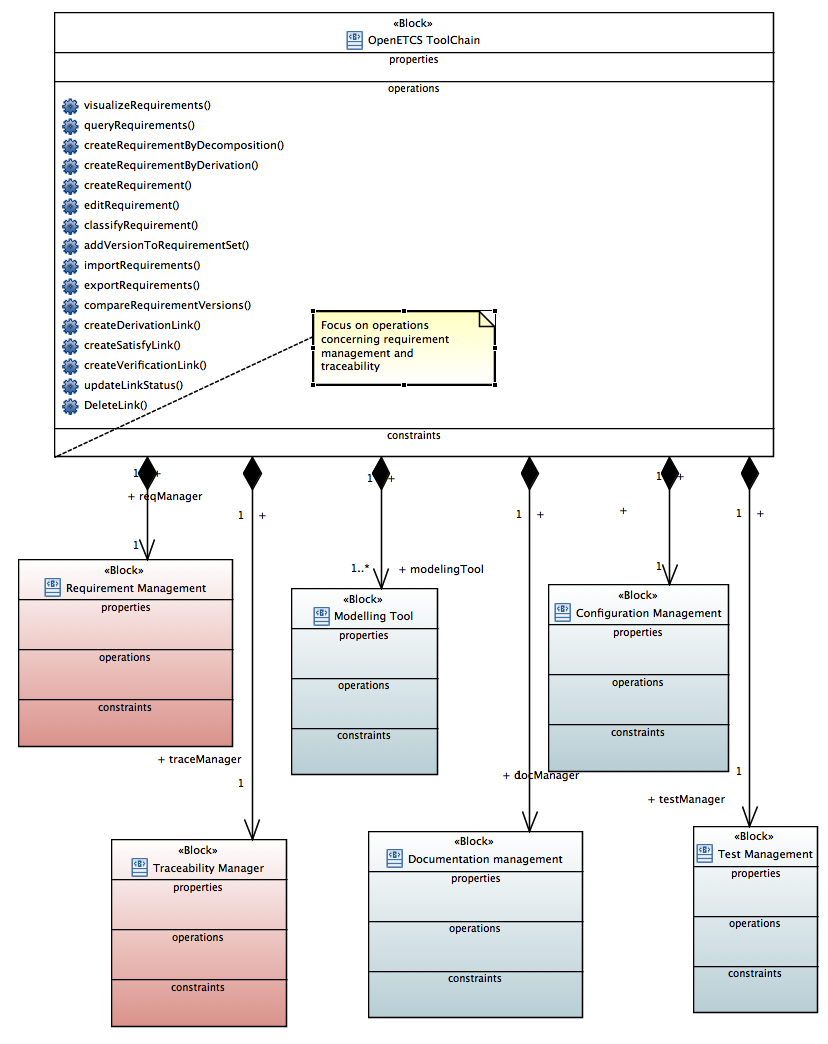
\includegraphics[width=.9\linewidth]{images/ToolChainLogicalArchitecture.png}
\caption{\label{fig:ToolChainLogicalArchitecture}Tool chain logical architecture with focus on requirement management and traceability}
\end{figure}

Figure \ref{fig:ToolChainWhiteBoxInteractionsConcerningTraceability} shows interactions between tool chain logical components concerning requirement flow down and traceability.


\begin{figure}[hbtp]
\centering
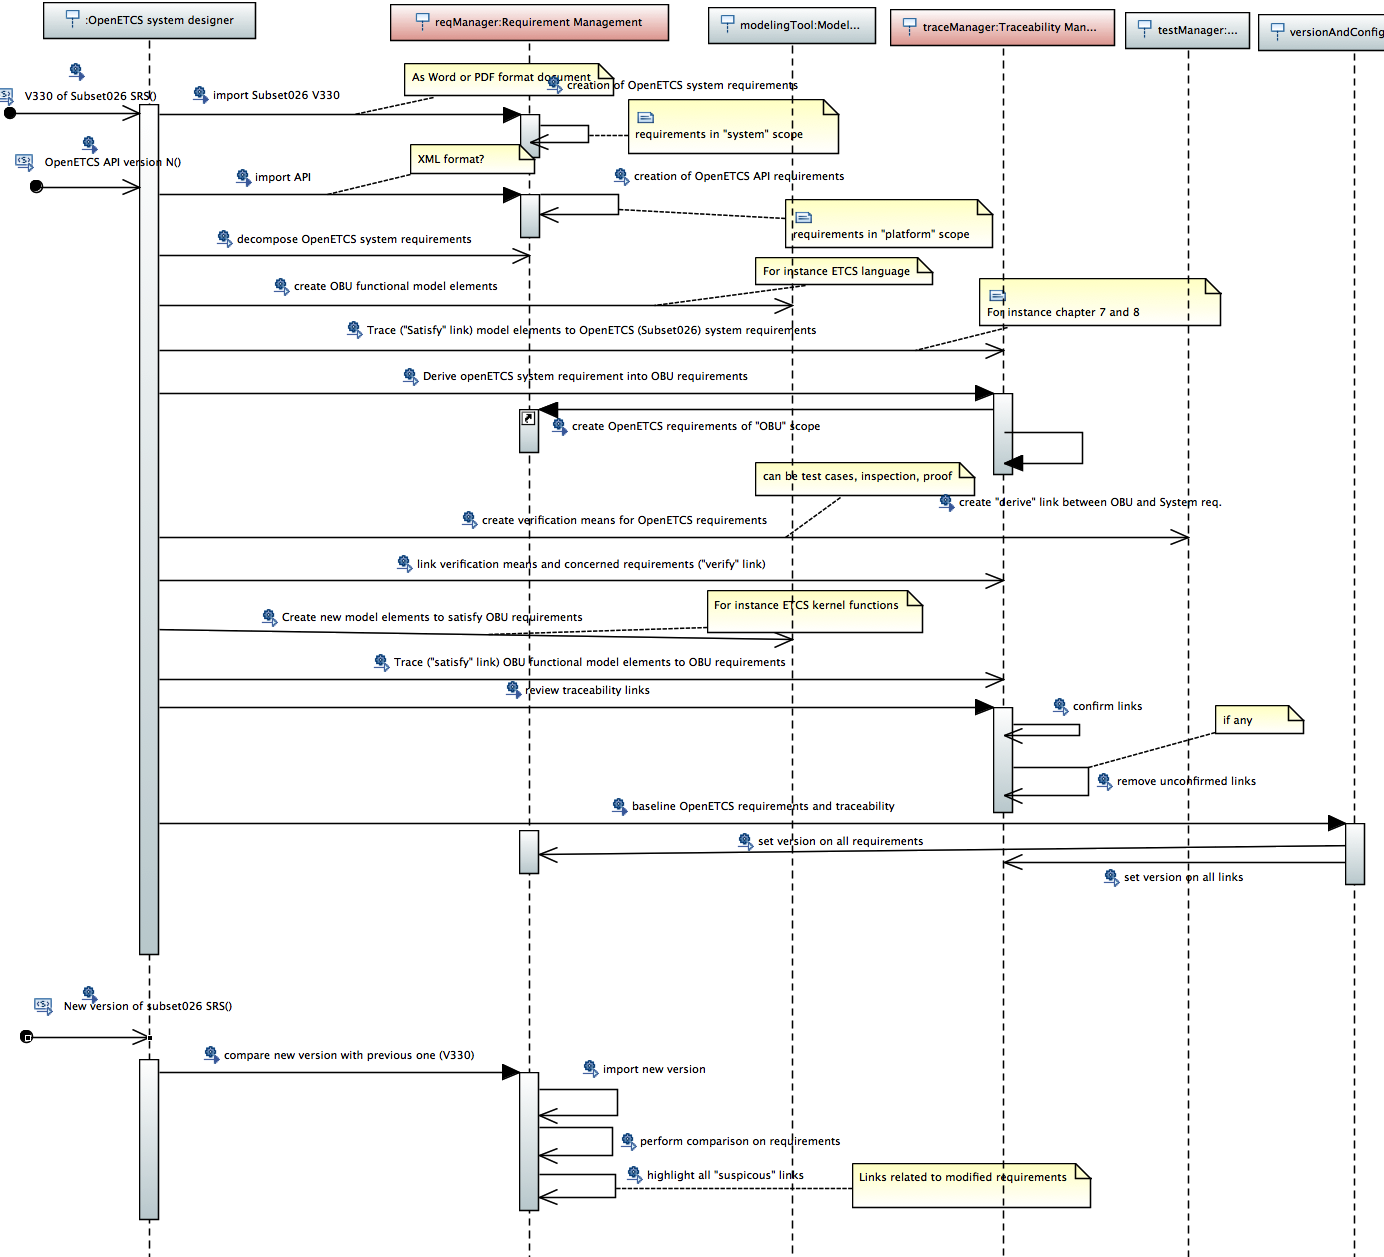
\includegraphics[width=1.1\linewidth]{images/ToolChainWhiteBoxInteractionsConcerningTraceability.png}
\caption{\label{fig:ToolChainWhiteBoxInteractionsConcerningTraceability}interaction between tool chain components to support requirement flow down and traceability}
\end{figure}

\section{Component design: existing technologies/tooling}

\subsection{Requirement management and traceability}
\label{sec-4-2} 
Concerning requirement management and traceability there exist a lot of solutions. If we focus on open source solutions and especially those able to integrate into Eclipse platform, we find:
\begin{itemize}
\item Eclipse Requirement Modeling Framework (RMF). As mentioned on Eclipse web site, RMF is a framework to manage textual requirements through ReqIF standard requirement exchange format. There is a powerful GUI called "ProR" to configure, visualize and edit ReqIF requirements in RMF.
RMF/ProR is the natural choice for OpenETCS to support requirement management.

Alternatively to deal with the closed source path the requirement management may
be done by Reqtify Gateway of SCADE (also called "RM Gateway"). 

ProR can also be used to support traceability between requirements (native functionality) and between requirements and Papyrus models through a "proxy" connector.

\item PolarSys ReqCycle. It is a solution that focuses on requirement traceability. It can allow managing requirements (creation, edition, queries) with classification (scopes) and custom requirement data models but with very limited requirement editor. Strength is its ability to capture and aggregate traceability links coming from different sources (EMF models, C code, Java code, SysML models...) and to define own traceability links based on custom link types with potential attributes.

\end{itemize}

If we extend search to proprietary solutions, we find IBM DOORS and IBM DOORS Next requirement management products and Dassault Systems ReqTify product as leading solutions to support respectively requirement management and requirement traceability.

\subsection{Modelling tool for system model}
The system model defines block and interfaces between those blocks that realize
the specification. This is done with Eclipse Papyrus. 

\subsection{Modelling tool for OBU functional model}
The system model defines block and interfaces between those blocks that realize
the specification. This is done with Eclipse Papyrus. 

\subsection{OBU Functional model}
\label{sec-10}
OBU functional model is done with SCADE suite tool.

\chapter{First physical traceability solution: ProR-RMGateway}
\label{sec-5}

This first solution consists in handling traceability "by hand" (without full integration in the tool chain), with different solutions locally integrated to the different modelling environments used in the project (SCADE and Papyrus) and aggregate results in a shared global requirement database.

\begin{figure}[htb]
\centering
\includegraphics[width=.9\linewidth]{images/first_trace_solution.pdf}
\caption{\label{fig:trace_first}Traceability architecture first solution}
\end{figure}

With that approach, there is one master reference requirements data base. This data
base is itself directly imported from the subset-026 word document. The data
base provides the list of requirements as well as an unique identifiers for each
requirement. These identifiers are fixed and cannot be modified by any other
tools. 

Note: it is possible for requirement management tools to complete imported
requirements but they should guarantee the following rules:
\begin{enumerate}
\item The requirement's structure (hierarchy, scope) is not modified.
\item No requirement should be deleted.
\item Newly added requirements should be either a refinement, derivation or a decomposition of an existing one.
\item The identifier pattern should be respected.
\item Identifiers should remain unique.
\end{enumerate}

Concerning database, best solution is to use ReqIF standard exchange format, as it can be fulfilled by most requirement management tools. 

Concerning requirement management and traceability "local" solutions we get: 
\begin{itemize}
\item For Scade modelling: most direct solution is Scade RM-Gateway (based on ReqTify solution) as it is integrated with SCADE tool.
Note: alternative solutions are "ReqCycle" (see other solutions later in this document).
\item For Papyrus SysML model: ProR can be used with a given proxy added to Papyrus to support creation of links between ReqIF requirements and SysML elements.
Note: another direct solution is to use ReqCycle solution that is well suited to create and capture links with Papyrus models. It will be investigated in another candidate architecture.

Figure \ref{fig:trace_first} illustrates this solution with associated tools/technologies.

\end{itemize}



\section{Subset-026 import}
\label{sec-5-1}
The subset-026 import is realized by a script transforming the Word document
into a req-IF format file.
\subsection{Script description}
\label{sec-5-1-1}
The script \todo{The script needs a name} generates a hierarchical tree of all traceworthy
artifacts in each chapter of subset-026. Each artifact shall be uniquely
addressable via a tracestring.


\subsection{Unique ID definition}
\label{sec-5-1-2}
Take the following example:
\begin{figure}[htb]
\centering
\includegraphics[width=.9\linewidth]{images/tracestring-ex.png}
\caption{\label{fig:reqID_ex}Traceability architecture between artifacts}
\end{figure}


\paragraph{Guideline}
The scope of a single requirement ID is a paragraph of text (there are six such
paragraphs in the above example).  requirement IDs are hierarchical. The
hierarchy is a direct mapping of the hierarchy in the original subset-026
text. Levels are separated by a dot. There is a requirement at each level
(i.e. you may truncate the requirement ID to any level and it stays valid).

\paragraph{How to}

Suppose we want to trace the fifth paragraph in the above example i.e
\begin{verbatim}
• End of mission is performed
\end{verbatim}
\begin{enumerate}
\item Let \textsl{traceString} be the variable to store the result.
\item Find the current running number of the base list. That is the list which
includes the chapter number. In this example this number equals
\verb+3.5.3.7.+ Set \textsl{traceString} to this number.
\item Count the number of paragraphs in this list item starting with 1 and append
this number in square brackets to the \textsl{traceString} if it is greater than 1.

Note: For the first iteration in the example there is only one such paragraph
(\texttt{If the establishment...}). Hence, we do not append anything. In the
second iteration there are two such paragraphs (\texttt{The on-board shall...} and
\texttt{If this request is not ...}). Hence, the second one will receive an
\texttt{[2]} appendix.

\item Until you arrived at your target paragraph: Append any running number of
sub-lists and remove leading or trailing characters (such as braces). If the
current sub-list is bulleted then the level string always becomes
\verb+[*][n]+ (with n being the running number of that bullet starting at
1). Prefix this new level with a dot (\verb+.+) and append it to the
\textsl{traceString}.

Note: \verb+a)+ is the identifier of one such sub-list item. The trailing brace
will be removed. The bullet points form another (less significant) sub-list.
\item Do step 3.
\item Do step 4 or break.
\item \textsl{traceString} is now the fully qualified requirementID.
\end{enumerate}

This will result in the following requirement ID: \quad \verb+3.5.3.7.a[2].[*][2]+



\section{System Model}
\label{sec-8}

The link with the requirement may be included via requirements diagram with a
direct link of requirement in ProR
The explanation to performs the link may be found here \href{https://github.com/openETCS/toolchain/wiki/User-Documentation#tracing-requirements-and-sysml-models}{ProR-Papyrus proxy}.
The links may be viewed through Papyrus an ProR and the requirement may be
directly apply from ProR to a Papyrus elements.


\section{Interface Definition}
\label{sec-9}

It should define the interfaces between the architecture artefacts.  It is used and
set up to facilitate team working together on a big architecture. Its definition
comes from the requirements but can also be refined by the modelling team without
changing the existing implemented requirements.



\section{{\bfseries\sffamily TODO} Verification and Validation}
\label{sec-11}

\chapter{Second physical traceability solution: ProR-ReqCycle}
\label{sec-6}

This second solution consists in using only one centralized Requirement database (as in solution 1) managed by one eclipse-based requirement management solution (ProR) and only one eclipse-based technology to support requirement traceability for all models (Papyrus and SCADE): PolarSys ReqCycle.

\begin{figure}[htb]
\centering
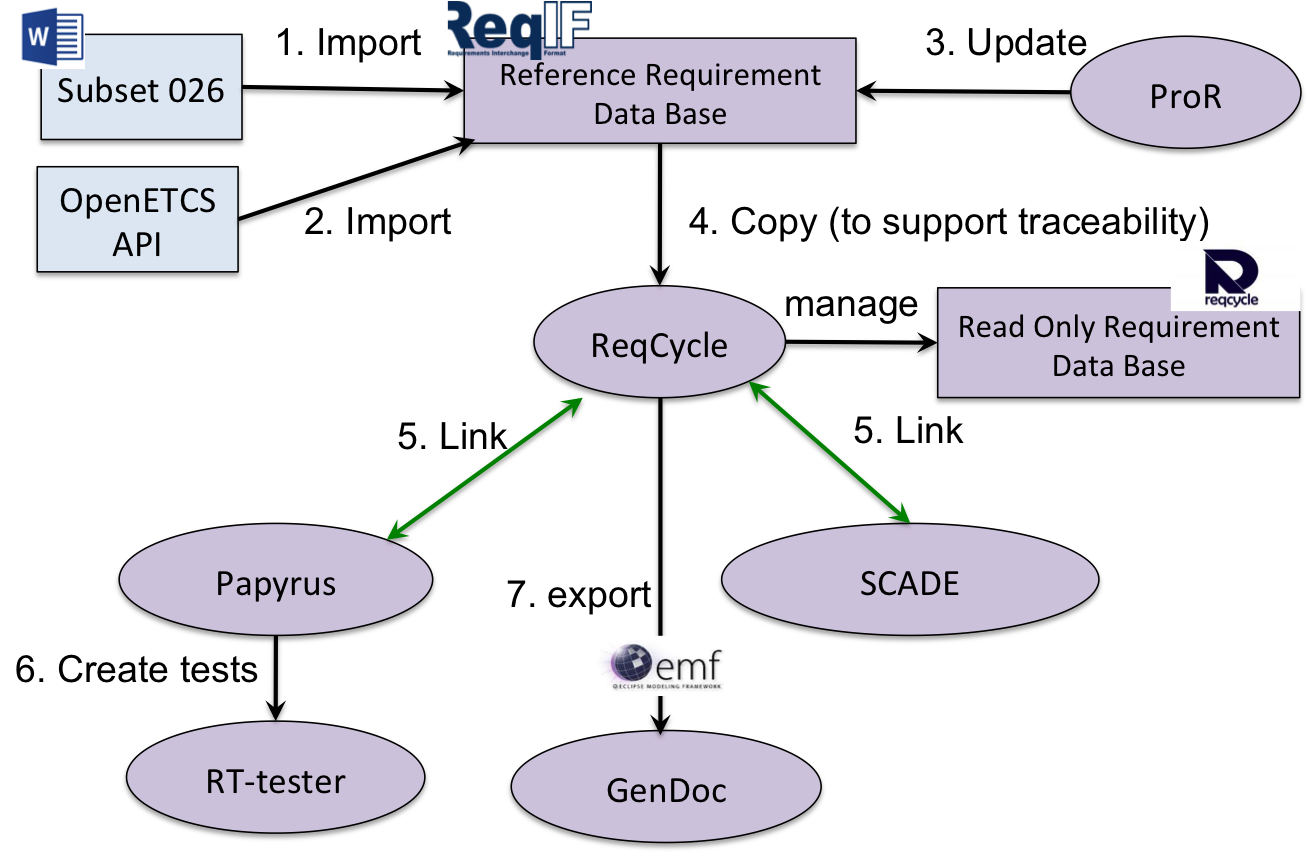
\includegraphics[width=.9\linewidth]{images/second_trace_solution-ProR-ReqCycle.png}
\caption{\label{fig:trace_second}Traceability architecture second solution}
\end{figure}

With that approach, there is still one master reference requirements data base entirely managed by ProR. Requirement database is initialized by import from the subset-026 word document, as in solution 1 (see \ref{sec-5-1}) and by import from OpenETCS API.
All new OpenETCS requirements are added in this requirement database through ProR tool.

Traceability is managed by ReqCycle tool. In order to ease visual selection of requirements in ReqCycle, there is a copy (could be a link) of reference requirements hierarchy into a ReqCycle database. Then ReqCycle manages links with Papyrus and links with SCADE. 
Finally, traceability can be exported by ReqCycle and processed by Gendoc tool to deliver documentation.

Most complex commands are detailed in next paragraphs.

\section{Subset-026 import}
\label{sec-6-1}
The subset-026 import can be realized by two means:
\begin{itemize}
\item either by direct import from the subset-026 word document (ReqCycle Document import connector)
\item else by a two steps process with transformation from word document to .ReqIF files (1.B1 path in the figure) and then import of those .ReqIF files into ReqCycle requirement database (1.B2 path).
	\begin{itemize}

	\item 1.A1 transformation can be realized with same script than the one described in first traceability solution - see \ref{sec-5-1}

	\item 1.A2 transformation (import) can be done by ReqCycle ReqIF import connector.
	\end{itemize}
\end{itemize}

\section{Creation of additional OpenETCS requirements}
\label{sec-6-2}
ProR can create new requirements by decomposition or by derivation of existing requirements.
In case of derivation, engineering level (scope) changes (for instance from System to OBU or to OBU Kernel).
Regularly, when there have been new requirements created, there must by a copy to the ReqCycle database so that ReqCycle can manage traceability to those requirements.

\textbf{Note}: in the future, we could have a link (reference) between ProR requirement database (ReqIF format) and ReqCycle database, rather than a copy. We could also have traceability created on requirement selected in ProR tool.

\section{Creation of links between SysML model elements and requirements}
\label{sec-6-3}
ReqCycle
ReqCycle provides a view that allows creating a link between two selected objects (traceability Creator).
ReqCycle provides a view with requirements (Requirement View) from which it is possible to select one source object.
Papyrus provides a view with model elements (Model explorer) from which it is possible to select a destination object.
When both source and destination objects are selected, ReqCycle provides a command (button) to create links between selected objects if a link type definition is compliant with such source and destination.

Figure to DO.

\section{Creation of links between SCADE model and requirements}
\label{sec-6-4}
There are two approaches that can be used: 
\begin{enumerate}
\item use same approach than in \ref{sec-6-3} but there is some development to make selection of SCADE model element appear in ReqCycle traceability creator view
\item select requirement in ReqCycle Requirement view and prepare the creation of traceability link through a dedicated ReqCycle command that copies the traceability link identifier in clipboard, and then use "paste" command in SCADE tool environement, in the comment area associated to the model element to trace.
\end{enumerate} 

Figure to DO.

\section{Aggregation of traceability links and export}
\label{sec-6-5}
It is done by ReqCycle that has all information (copy of the requirement database and associated traceability between requirements + all traceability links with models).
It is exported into EMF format that can be processed by Gendoc to render expected documentation including traceability.

\chapter{Third physical traceability solution: ReqCycle}
\label{sec-7}
This third solution consists in using only one centralized Requirement database (as in previous solutions) managed by one eclipse-based solution (ReqCycle) also used to support requirement traceability for all models (Papyrus and SCADE).

\begin{figure}[htb]
\centering
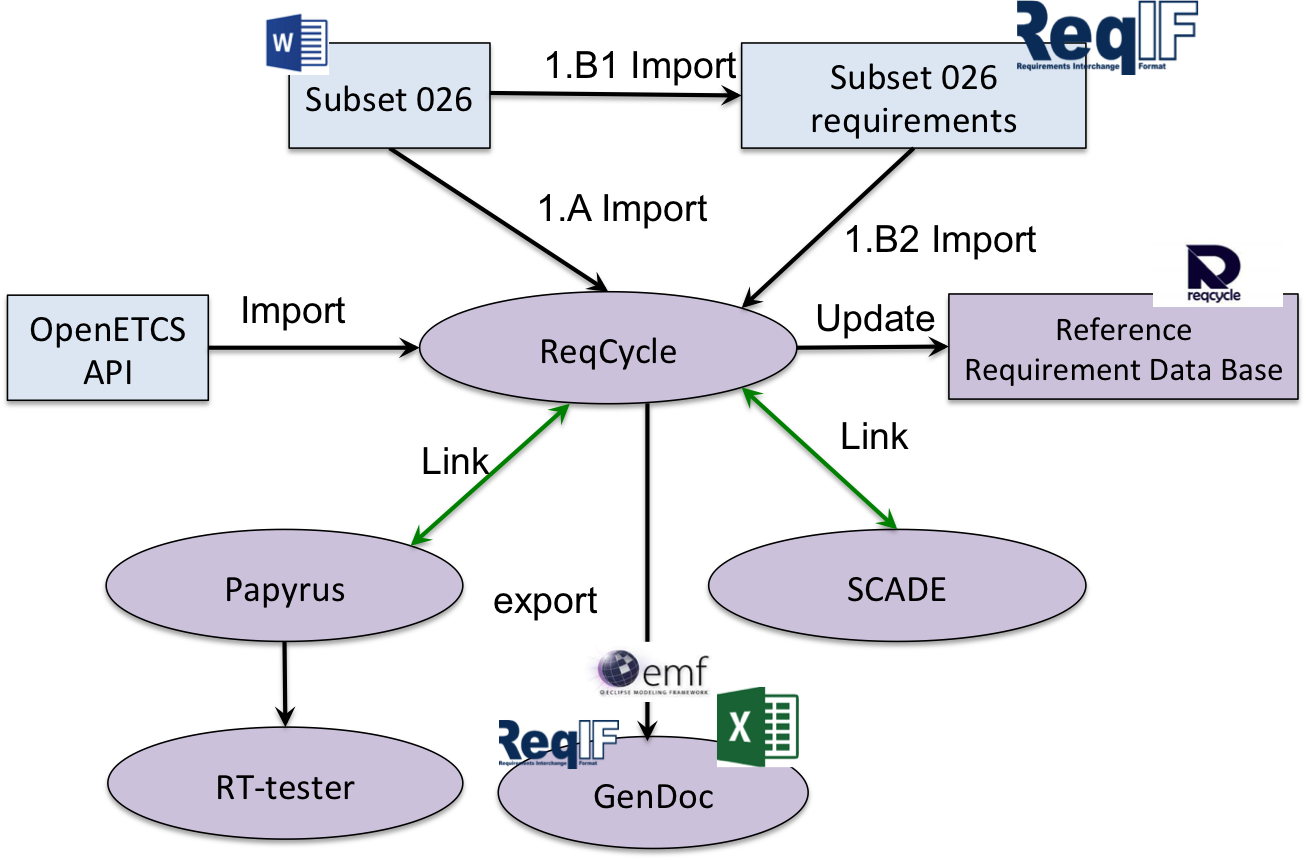
\includegraphics[width=.9\linewidth]{images/Third-Solution-ReqCycle.png}
\caption{\label{fig:trace_third}Traceability architecture third solution with ReqCycle only}
\end{figure}

With that approach, there is still one master reference requirements data base entirely managed by ReqCycle. Requirement database is initialized by import from the subset-026 word document through two possible means (see next section) and by import from OpenETCS API.
All new OpenETCS requirements are added in this requirement database through ReqCycle tool.

Traceability is managed by ReqCycle tool. In order to ease visual selection of requirements in ReqCycle, there is a copy (could be a link) of reference requirements hierarchy into a ReqCycle database. Then ReqCycle manages links with Papyrus and links with SCADE. 
Finally, traceability can be exported by ReqCycle and processed by Gendoc tool to deliver documentation.

Most complex commands are detailed in next paragraphs.


\section{Subset-026 import}
\label{sec-7-1}
The subset-026 import can be realized by two means:
\begin{itemize}
\item either by direct import from the subset-026 word document (ReqCycle Document import connector)
\item else by a two steps process with transformation from word document to .ReqIF files (1.B1 path in the figure) and then import of those .ReqIF files into ReqCycle requirement database (1.B2 path).
	\begin{itemize}

	\item 1.A1 transformation can be realized with same script than the one described in first traceability solution - see \ref{sec-5-1}

	\item 1.A2 transformation (import) can be done by ReqCycle ReqIF import connector.
	\end{itemize}
\end{itemize}

\section{Creation of additional OpenETCS requirements}
\label{sec-7-2}
ReqCycle provides a "local" connector to create new requirements and those requirements can be linked to existing other requirements through different kinds of links (derivation, refinement, decomposition). Those link types have to be defined first in ReqCycle configuration.

To complete

\section{Creation of links between SysML model elements and requirements}
\label{sec-7-3}
Same solution than in second solution. see \ref{sec-6-3}

\section{Creation of links between SCADE model and requirements}
\label{sec-6-4}
Same solution than in second solution. see \ref{sec-6-4}

\section{Aggregation of traceability links and export}
\label{sec-6-5}
Same solution than in second solution. see \ref{sec-6-5}



\chapter{Tool evaluations}
\subsection{{\bfseries\sffamily TODO} ReqCycle  Evaluation}
\label{sec-4-5}
\subsection{{\bfseries\sffamily TODO} Reqtify Evaluation}
\label{sec-4-6}



% Emacs 24.3.1 (Org mode 8.2.4)
\end{document}

%%  LocalWords:  traceability OpenETCS
